\sect{Section 1 - Invited Talks} \label{Sect1}
%HSL: I have moved this to the intro
%This section contains a reflection on each of the invited talks in the light of the hypothesis of this report. Full notes from the lectures have been recorded in Appendix 4.


\phantomsection
\addcontentsline{toc}{subsection}{Domino Printing Sciences PLC}
\subsect{Domino Printing Sciences PLC - Carl Reynaud - Director of Hardware Development}
%Overview of each of the talks and an assessment of the information presented in light of the report topic 'How does technology make profit?' 
Domino Printing Sciences PLC designs, manufactures and markets a range of printing equipment for a wide range of applications \cite{DominoAnnual}. 
In 2013 Domino achieved a global turnover of \textsterling335.7m from operations in over 120 countries \cite{DominoFactsheet}. 
Domino was founded in 1978 \cite{DominoFactsheet} as a spin out following a project at technology consultancy Cambridge Consultants.
Graeme Minto led the project developing continuous inkjet (CIJ) technology, and consequently founded Domino Printing Sciences following the departure of the project's client \cite{goffin2010innovation}.
This is an example of a company starting with a core technological innovation as the focus, as asserted by Johnson in \cite{ johnson2008exploring}.

By the mid-90s CIJ was reaching technological limits of exploitation. 
Despite the many advantages of the technology, customers wanted higher resolution images in bigger sizes than were possible with CIJ. Hence Domino began an extensive review of alternative technologies including laser printing, `binary' inkjet and `drop-on-demand' technology.
During the 90s, Domino built on the expertise built from CIJ technology to expand and diversify to become a multi-technology company. 
This diversification into other related technologies have enabled Domino to retain their existing customer base while entering new and emerging markets \cite{goffin2010innovation}.
Instead of just printing date codes, Domino has diversified into technologies to print patterns for laminates, ceramic floor tiles, complex food labels, cable labelling and more.
This is an example of a company adopting related diversification as a corporate strategy, enabling continued and extensive profit from technology.



\subsect{ARM - John Biggs - Consultant Engineer and Co-Founder}
%Overview of each of the talks and an assessment of the information presented in light of the report topic 'How does technology make profit?' 
ARM was founded in 1990 in Cambridge, U.K. as a result of a joint venture between Apple, Acorn and VLSI.
The primary function of ARM was to design processor architectures, but not to manufacture them.
ARM's business model involved the licensing of architectures, as opposed to the sale. 
This also included income from royalties which funded the next products.
They are now the world's leading semiconductor IP company and have shipped 50 billion devices to date.

ARM were able to grasp the low power market ahead of larger CPU firms such as Intel. 
This gave ARM an advantage in the mobile age as it increased battery life of smartphones and tablets.

Although ARM mainly design CPUs, there is still a large amount of diversity within their product range.
In 1997, the company expanded into memory, video and I/O controllers to support the processors.
Latest processors can be found in a range of devices, from $mm^{3}$ sized devices, to $km^{3}$ sized. 
ARM is also currently expanding into the microserver market.
This related diversity, although in very similar areas, resulted in ARM being a resounding success.



\subsect{Imagination Technologies - Dr David Knox - Senior Director Software Engineering}

Imagination technologies started off as Video Logic in 1985 but shifted towards an IP licensing company in 1999 eventually becoming a leading company in silicon, software and cloud technology~\cite{ImgHist}.
The company also has interesting sideline, inspired by their beginnings in audio, they design and build digital radios.
Using this profitable outlet as a substrate to showcase their chip designs allows them to gain feedback from the customer.
The business model held in figure~\ref{figure:ImgModel} is a multi-year cycle in which the Imagination see themselves as using customer feedback to drive chip development for licensees and also advising manufacturers on what's needed for emerging markets. 


\begin{figure}[htb]
   \centering
   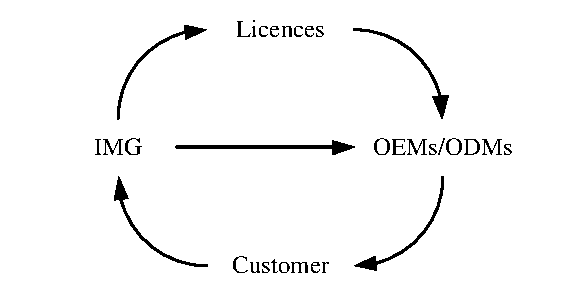
\includegraphics[width = 0.45\textwidth]{figures/ImgModel.pdf}
   \label{figure:ImgModel}
   \caption{Imagination technologies business model.}
\end{figure}



\subsect{Reflection on Common Themes}
The full content of the invited talks is given in Appendix 5. 
The shorter summaries given in this section have highlighted some elements of common strategy.
Each of these companies started with a technological core focus.
This technical excellence or key innovation often has an integral role in the early company stages.
However, these companies are now well established and have since expanded and diversified into new areas.
These new markets and products are often related to the core technical competence of the initial business.
This allows the company to exploit their core competencies in other markets, increasing the profit potential of the company.
With these thoughts in mind, Section 2 examines further case studies of established companies to build a body of evidence for the claim that related diversification is the key to profitability.



